\chapter{Arrays}
\label{chap10}
\label{arrays}
\index{array}
\index{type!array}

An {\bf array} is a set of values where each value is identified by an
index.  You can make an array of {\tt int}s, {\tt double}s, or any
other type, but all the values in an array have to have the same type.

Syntactically, array types look like other Java types except they are
followed by {\tt []}.  For example, {\tt int[]} is the type ``array of
integers'' and {\tt double[]} is the type ``array of doubles.''

You can declare variables with these types in the usual ways:

\begin{code}
    int[] count;
    double[] values;
\end{code}

Until you initialize these variables, they are set to {\tt null}.
To create the array itself, use {\tt new}.

\begin{code}
    count = new int[4];
    values = new double[size];
\end{code}

The first assignment makes {\tt count} refer to an array of 4
integers; the second makes {\tt values} refer to an array of {\tt
double}s.  The number of elements in {\tt values} depends on {\tt
size}.  You can use any integer expression as an array
size.

\index{null}
\index{state diagram}

The following figure shows how arrays are represented in state
diagrams:


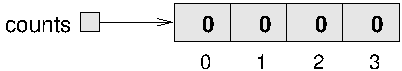
\includegraphics{figs/array.pdf}


The large numbers inside the boxes are the {\bf elements} of
the array.  The small numbers outside the boxes are the
indices used to identify each box.  When you allocate an
array if {\tt int}s, the elements are initialized to zero.


\section{Accessing elements}
\index{element}
\index{array!element}

To store values in the array, use the
{\tt []} operator.  For example {\tt count[0]} refers to the
``zeroeth'' element of the array, and {\tt count[1]} refers to the
``oneth'' element.  You can use the {\tt []} operator anywhere in an
expression:

\begin{code}
    count[0] = 7;
    count[1] = count[0] * 2;
    count[2]++;
    count[3] -= 60;
\end{code}

These are all legal assignment statements.  Here is the
result of this code fragment:


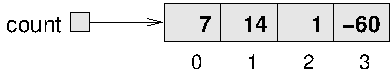
\includegraphics{figs/array2.pdf}


The elements of the array
are numbered from 0 to 3, which means that there is no element with
the index 4.  This should sound familiar, since we saw the same thing
with {\tt String} indices.  Nevertheless, it is a common error to go
beyond the bounds of an array, which throws an {\tt
ArrayOutOfBoundsException}.
\index{exception!ArrayOutOfBounds}
\index{run-time error}
\index{index}

You can use any expression as an index, as long as it has type {\tt
int}.  One of the most common ways to index an array is with a loop
variable.  For example:
\index{expression}

\begin{code}
    int i = 0;
    while (i < 4) {
        System.out.println(count[i]);
        i++;
    }
\end{code}

This is a standard {\tt while} loop that counts from 0
up to 4, and when the loop variable {\tt i} is 4, the
condition fails and the loop terminates.  Thus, the body
of the loop is only executed when {\tt i} is 0, 1, 2 and 3.

\index{loop}
\index{loop variable}
\index{variable!loop}

Each time through the loop we use {\tt i} as an index into
the array, printing the {\tt i}th element.  This type of
array traversal is very common.


\section{Copying arrays}
\index{array!copying}

When you copy an array variable, remember that you are
copying a reference to the array.  For example:

\begin{code}
    double[] a = new double [3];
    double[] b = a;
\end{code}

This code creates one array of three {\tt double}s, and
sets two different variables to refer to it.
This situation is a form of aliasing.


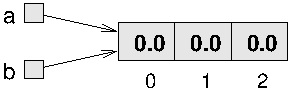
\includegraphics{figs/array3.pdf}


Any changes in either array
will be reflected in the other.  This is not usually the
behavior you want; more often you want to
allocate a new array and copy elements from
one to the other.

\begin{code}
    double[] b = new double [3];

    int i = 0;
    while (i < 4) {
      b[i] = a[i];
      i++;
    }
\end{code}


\section{Arrays and objects}
\index{object!compared to array}
\index{array!compared to object}

In many ways, arrays behave like objects:

\begin{itemize}

\item When you declare an array variable, you get a reference
to an array.

\item You have to use {\tt new} to create the array itself.

\item When you pass an array as an argument, you pass a reference,
which means that the invoked method can change the contents
of the array.

\end{itemize}

Some of the objects we looked at, like {\tt Rectangles}, are
similar to arrays in the sense that they are collections of
values.  This raises the question, ``How is an array of 4 integers
different from a Rectangle object?''
\index{collection}

If you go back to the definition of ``array'' at the beginning
of the chapter, you see one difference: the
elements of an array are identified by indices, and the
elements of an object have names.

Another difference is that the
elements of an array have to be the same type.  Objects can
have instance variables with different types.


\section{{\tt for} loops}
\label{for}

The loops we have written have a number of elements
in common.  All of them start by initializing a variable;
they have a test, or condition, that depends on that variable;
and inside the loop they do something to that variable,
like increment it.

\index{loop!for}
\index{for}
\index{statement!for}

This type of loop is so common that there is another
loop statement, called {\tt for}, that expresses it more
concisely.  The general syntax looks like this:

\begin{code}
    for (INITIALIZER; CONDITION; INCREMENTOR) {
        BODY
    }
\end{code}

This statement is equivalent to

\begin{code}
    INITIALIZER;
    while (CONDITION) {
        BODY
        INCREMENTOR
    }
\end{code}

except that it is more concise and, since it puts all the
loop-related statements in one place, it is easier to read.
For example:

\begin{code}
    for (int i = 0; i < 4; i++) {
        System.out.println(count[i]);
    }
\end{code}

is equivalent to

\begin{code}
    int i = 0;
    while (i < 4) {
        System.out.println(count[i]);
        i++;
    }
\end{code}


\section{Array length}
\index{length!array}
\index{array!length}

All arrays have one named instance variable: {\tt length}.
Not surprisingly, it contains the length of the array (number
of elements).  It is a good idea to use this value as the upper
bound of a loop, rather than a constant value.  That way, if
the size of the array changes, you won't have to go through the
program changing all the loops; they will work correctly for any
size array.

\begin{code}
    for (int i = 0; i < a.length; i++) {
        b[i] = a[i];
    }
\end{code}

The last time the body of the loop gets executed, {\tt i}
is {\tt a.length - 1}, which is the index of the last element.  When
{\tt i} is equal to {\tt a.length}, the condition fails and the body
is not executed, which is a good thing, since it would throw an
exception.  This code assumes that the array {\tt b} contains at least
as many elements as {\tt a}.


\section{Random numbers}
\label{random}
\label{pseudorandom}
\index{random number}
\index{deterministic}
\index{nondeterministic}

Most computer programs do the same thing every time they are executed,
so they are said to be {\bf deterministic}.  Usually, determinism is a
good thing, since we expect the same calculation to yield the same
result.  But for some applications we want the
computer to be unpredictable.  Games are an obvious example, but
there are more.

Making a program truly {\bf nondeterministic} turns out to be not so
easy, but there are ways to make it at least seem nondeterministic.
One of them is to generate random numbers and use them to determine
the outcome of the program.  Java provides a method that generates
{\bf pseudorandom} numbers, which may not be truly random, but for our
purposes, they will do.

Check out the documentation of the {\tt random} method in the {\tt
Math} class.  The return value is a {\tt double} between 0.0 and 1.0.
To be precise, it is greater than or equal to 0.0 and strictly less
than 1.0.  Each time you invoke {\tt random} you get the next
number in a pseudorandom sequence.
To see a sample, run this loop:

\begin{code}
    for (int i = 0; i < 10; i++) {
        double x = Math.random();
        System.out.println(x);
    }
\end{code}

To generate a random {\tt double} between 0.0 and an upper bound like
{\tt high}, you can multiply {\tt x} by {\tt high}.


\section{Array of random numbers}
\label{randarray}

How would you generate a random integer between {\tt low} and {\tt high}?
If your implementation of {\tt randomInt} is correct, then
every value in the range from {\tt low} to {\tt high-1} should
have the same probability.  If you generate a long series
of numbers, every value should appear, at least approximately,
the same number of times.

One way to test your method is to
generate a large number of random values,
store them in an array, and count the number of times each
value occurs.

The following method takes a single argument, the size of
the array.  It allocates a new array of integers, fills
it with random values, and returns a reference to the new
array.

\begin{code}
  public static int[] randomArray(int n) {
      int[] a = new int[n];
      for (int i = 0; i<a.length; i++) {
          a[i] = randomInt(0, 100);
      }
      return a;
  }
\end{code}

The return type is {\tt int[]}, which means that
this method returns an array of integers.
To test this method, it is convenient to have a method that
prints the contents of an array.

\begin{code}
  public static void printArray(int[] a) {
      for (int i = 0; i<a.length; i++) {
          System.out.println(a[i]);
      }
  }
\end{code}

The following code generates an array and prints it:

\begin{code}
    int numValues = 8;
    int[] array = randomArray(numValues);
    printArray(array);
\end{code}

On my machine the output is

\begin{stdout}
27
6
54
62
54
2
44
81
\end{stdout}

which is pretty random-looking.  Your results may differ.

If these were exam scores (and they would be pretty bad exam
scores) the teacher might present the results to the class
in the form of a {\bf histogram}, which is a set of counters
that keeps track of the number of times each value appears.

\index{histogram}

For exam scores, we might have ten counters to keep track of
how many students scored in the 90s, the 80s, etc.  The next
few sections develop code to generate a histogram.


\section{Counting}
\index{traverse!array}
\index{array!traverse}
\index{looping and counting}
\index{counter}

A good approach to problems like this is to think of simple methods
that are easy to write, then combine them into a solution.
This process is called {\bf bottom-up development}.
See \url{http://en.wikipedia.org/wiki/Top-down_and_bottom-up_design}.
\index{program development}

It is not always obvious where to start,
but a good approach is to look for subproblems that fit a pattern you
have seen before.

In Section~\ref{loopcount} we saw a loop that traversed a
string and counted the number of times a given letter appeared.  You
can think of this program as an example of a pattern called ``traverse
and count.''  The elements of this pattern are:

\begin{itemize}

\item A set or container that can be traversed, like an array
or a string.

\item A test that you can apply to each element in the container.

\item A counter that keeps track of how many elements pass
the test.

\end{itemize}

In this case, the container is an array of integers.  The
test is whether or not a given score falls in a given range of
values.

Here is a method called {\tt inRange} that counts the number of
elements in an array that fall in a given range.  The parameters are
the array and two integers that specify the lower and upper bounds of
the range.

\begin{code}
public static int inRange(int[] a, int low, int high) {
    int count = 0;
    for (int i = 0; i < a.length; i++) {
        if (a[i] >= low && a[i] < high) count++;
    }
    return count;
}
\end{code}

I wasn't specific about whether something equal
to {\tt low} or {\tt high} falls in the range, but you can
see from the code that {\tt low} is in and {\tt high} is out.
That keeps us from counting any elements twice.

Now we can count the number of scores in the ranges we are
interested in:

\begin{code}
int[] scores = randomArray(30);
int a = inRange(scores, 90, 100);
int b = inRange(scores, 80, 90);
int c = inRange(scores, 70, 80);
int d = inRange(scores, 60, 70);
int f = inRange(scores, 0, 60);
\end{code}


\section{The histogram}
\index{range}
\index{histogram}

This code is repetitious, but it is acceptable as
long as the number of ranges is small.  But imagine that
we want to keep track of the number of times each score appears,
all 100 possible values.  Would you want to write this?

\begin{code}
int count0 = inRange(scores, 0, 1);
int count1 = inRange(scores, 1, 2);
int count2 = inRange(scores, 2, 3);
...
int count3 = inRange(scores, 99, 100);
\end{code}

I don't think so.  What we really want is a way to store 100 integers,
preferably so we can use an index to access each one.  Hint: array.

The counting pattern is the same whether we use a single counter or an
array of counters.  In this case, we initialize the array outside the
loop; then, inside the loop, we invoke {\tt inRange} and store the
result:

\begin{code}
    int[] counts = new int[100];

    for (int i = 0; i < counts.length; i++) {
        counts[i] = inRange(scores, i, i+1);
    }
\end{code}

The only tricky thing here is that we are using the loop variable
in two roles: as in index into the array, and as the parameter to
{\tt inRange}.


\section{A single-pass solution}
\label{singlepass}

This code works, but it is not as efficient as it could
be.  Every time it invokes {\tt inRange}, it traverses the
entire array.  As the number of ranges increases, that gets
to be a lot of traversals.

It would be better to make a single pass through the array,
and for each value, compute which range it falls in.  Then
we could increment the appropriate counter.
In this example, that computation is trivial, because we
can use the value itself as an index into the array of counters.

Here is code that traverses an array of scores once and generates
a histogram.

\begin{code}
    int[] counts = new int[100];

    for (int i = 0; i < scores.length; i++) {
        int index = scores[i];
        counts[index]++;
    }
\end{code}


\section{Glossary}

\begin{description}

\item[array:]  A collection of values, where all the
values have the same type, and each value is identified by
an index.

\item[element:]  One of the values in an array.  The {\tt []}
operator selects elements.

\item[index:]  An integer variable or value used to indicate
an element of an array.

\item[deterministic:]  A program that does the same thing every
time it is invoked.

\item[pseudorandom:]  A sequence of numbers that appear to be
random, but which are actually the product of a deterministic
computation.

\item[histogram:]  An array of integers where each integer
counts the number of values that fall into a certain range.

\index{array}
\index{element}
\index{index}
\index{deterministic}
\index{pseudorandom}

\end{description}


\section{Exercises}

\begin{exercise}
Write a method called {\tt cloneArray} that takes an
array of integers as a parameter, creates a new array that is the same
size, copies the elements from the first array into the new one, and
then returns a reference to the new array.
\end{exercise}


\begin{exercise}
Write a method called {\tt randomDouble} that takes two doubles,
{\tt low} and {\tt high}, and that returns a random double $x$
so that $low \le x < high$.
\end{exercise}


\begin{exercise}
\label{ex.randint}
Write a method called {\tt randomInt} that takes two arguments,
{\tt low} and {\tt high}, and that returns a random integer between
{\tt low} and {\tt high}, not including {\tt high}.
\end{exercise}


\begin{exercise}
Encapsulate the code in Section~\ref{singlepass} in a method called
{\tt makeHist} that takes an array of scores and returns a histogram
of the values in the array.
\end{exercise}


\begin{exercise}
Write a method named {\tt areFactors} that takes
an integer {\tt n} and an array of integers, and that returns
{\tt true} if the numbers in the array are all factors of {\tt n}
(which is to say that {\tt n} is divisible by all of them).
HINT: See Exercise~\ref{ex.isdiv}.
\end{exercise}


\begin{exercise}
Write a method that takes an array of integers and an integer named
{\tt target} as arguments, and that returns the first index where
{\tt target} appears in the array, if it does, and -1 otherwise.
\end{exercise}


\begin{exercise}
Some programmers disagree with the general rule that variables
and methods should be given meaningful names.  Instead, they
think variables and methods should be named after fruit.

For each of the following methods, write one sentence that
describes abstractly what the method does.  For each variable,
identify the role it plays.

\begin{code}
public static int banana(int[] a) {
    int grape = 0;
    int i = 0;
    while (i < a.length) {
        grape = grape + a[i];
        i++;
    }
    return grape;
}

public static int apple(int[] a, int p) {
    int i = 0;
    int pear = 0;
    while (i < a.length) {
        if (a[i] == p) pear++;
        i++;
    }
    return pear;
}

public static int grapefruit(int[] a, int p) {
    for (int i = 0; i<a.length; i++) {
        if (a[i] == p) return i;
    }
    return -1;
}
\end{code}

The purpose of this exercise is to practice reading code and
recognizing the computation patterns we have seen.
\end{exercise}


\begin{exercise}
\begin{enumerate}

\item What is the output of the following program?

\item Draw a stack diagram that shows the state of the
program just before {\tt mus} returns.

\item Describe in a few words what {\tt mus} does.
\end{enumerate}

\begin{code}
public static int[] make(int n) {
    int[] a = new int[n];

    for (int i = 0; i < n; i++) {
        a[i] = i+1;
    }
    return a;
}

public static void dub(int[] jub) {
    for (int i = 0; i < jub.length; i++) {
        jub[i] *= 2;
    }
}

public static int mus(int[] zoo) {
    int fus = 0;
    for (int i = 0; i < zoo.length; i++) {
        fus = fus + zoo[i];
    }
    return fus;
}

public static void main(String[] args) {
    int[] bob = make(5);
    dub(bob);

    System.out.println(mus(bob));
}
\end{code}
\end{exercise}


\begin{exercise}
Many of the patterns we have seen for traversing arrays can
also be written recursively.  It is not common to do so, but
it is a useful exercise.

\begin{enumerate}

\item Write a method called {\tt maxInRange} that takes an array of
integers and a range of indices ({\tt lowIndex} and {\tt highIndex}),
and that finds the maximum value in the array, considering only the
elements between {\tt lowIndex} and {\tt highIndex}, including both
ends.

This method should be recursive.  If the length of the range is 1,
that is, if {\tt lowIndex == highIndex}, we know immediately that the
sole element in the range must be the maximum.  So that's the base
case.

If there is more than one element in the range, we can break the array
into two pieces, find the maximum in each of the pieces, and then find
the maximum of the maxima.

\item Methods like {\tt maxInRange} can be awkward to use.  To
find the largest element in an array, we have to provide a range
that includes the entire array.

\begin{code}
    double max = maxInRange(array, 0, a.length-1);
\end{code}

Write a method called {\tt max} that takes an array as a parameter
and that uses {\tt maxInRange} to find and return the largest value.
Methods like {\tt max} are sometimes called {\bf wrapper methods}
because they provide a layer of abstraction around an awkward method
and make it easier to use.  The method that actually
performs the computation is called the {\bf helper method}.

\item Write a recursive version of {\tt find} using the
wrapper-helper pattern.  {\tt find} should take an array of
integers and a target integer.  It should return the index
of the first location where the target integer appears in the
array, or -1 if it does not appear.

\end{enumerate}
\end{exercise}

\begin{exercise}
One not-very-efficient way to sort the elements of an array
is to find the largest element and swap it with the first
element, then find the second-largest element and swap it with
the second, and so on.  This method is called a {\bf selection
sort} (see \url{http://en.wikipedia.org/wiki/Selection_sort}).

\begin{enumerate}

\item Write a method called {\tt indexOfMaxInRange} that
takes an array of integers, finds the
largest element in the given range, and returns its {\em index}.
You can modify your recursive version of {\tt maxInRange} or
you can write an iterative version from scratch.

\item Write a method called {\tt swapElement} that takes an
array of integers and two indices, and that swaps the elements
at the given indices.

\item Write a method called {\tt selectionSort} that takes an array of
integers and that uses {\tt indexOfMaxInRange} and {\tt swapElement}
to sort the array from largest to smallest.

\end{enumerate}
\end{exercise}


\begin{exercise}
Write a method called {\tt letterHist} that takes a String as a
parameter and that returns a histogram of the letters in the String.
The zeroeth element of the histogram should contain the number of a's
in the String (upper and lower case); the 25th element should contain
the number of z's.
Your solution should only traverse the String once.
\end{exercise}


\begin{exercise}
A word is said to be a ``doubloon'' if every letter that appears in the
word appears exactly twice.  For example, the following are all the
doubloons I found in my dictionary.

\begin {quote}
Abba, Anna, appall, appearer, appeases, arraigning, beriberi,
bilabial, boob, Caucasus, coco, Dada, deed, Emmett, Hannah,
horseshoer, intestines, Isis, mama, Mimi, murmur, noon, Otto, papa,
peep, reappear, redder, sees, Shanghaiings, Toto
\end{quote}

Write a method called {\tt isDoubloon} that returns {\tt true}
if the given word is a doubloon and {\tt false} otherwise.
\end{exercise}


\begin{exercise}
Two words are anagrams if they contain the same letters (and the
same number of each letter).  For example, ``stop'' is an anagram
of ``pots'' and ``allen downey'' is an anagram of ``well annoyed.''

Write a method that takes two Strings and returns {\tt true} if
the Strings are anagrams of each other.

Optional challenge: read the letters of the Strings only once.
\end{exercise}


\begin{exercise}
In Scrabble each player has a set of tiles with letters on them, and
the object of the game is to use those letters to spell words.  The
scoring system is complicated, but longer words are usually
worth more than shorter words.

Imagine you are given your set of tiles as a String, like {\tt
"quijibo"} and you are given another String to test, like {\tt "jib"}.
Write a method called {\tt canSpell} that takes two Strings and
returns {\tt true} if the set of tiles can be used to spell the word.  You
might have more than one tile with the same letter, but you can only
use each tile once.

Optional challenge: read the letters of the Strings only once.
\end{exercise}


\begin{exercise}
In real Scrabble, there are some blank tiles that can be used
as wild cards; that is, a blank tile can be used to represent
any letter.

Think of an algorithm for {\tt canSpell} that deals with wild
cards.  Don't get bogged down in details of implementation like
how to represent wild cards.  Just describe the algorithm, using
English, pseudocode, or Java.
\end{exercise}



